\documentclass[twocolumn]{article}
\usepackage[margin=1in]{geometry}
\usepackage{graphicx}
\graphicspath{ {C:/John/LaTeX/Scioly/Thermo/images/} }
\usepackage{grffile}
\usepackage{amsmath}

\title{Thermodynamics Event Guide}
\author{John Yang, Dylan Herrera}
\date{March 22, 2019}

\begin{document}

\twocolumn[
\begin{@twocolumnfalse}
\maketitle
\begin{abstract}
Thermodynamics was a Science Olympiad event in '17-'18 and '18-'19. Although it will be rotating out for the 2020 school year, it may return sooner or later, so feel free to use this guide. This event focuses on the science of thermodynamics, which is an intriguing bridge between physics and chem. The event encompasses two major parts: 1) design, construction and calibration of an insulating device, and 2) a written test on thermodynamics. 
\end{abstract}
\end{@twocolumnfalse}
]

\section{Device Testing}
Participants will construct an insulating device for a 250 mL beaker of hot water. For div. C, the maximum allowed dimensions were $15\times15\times15$cm, for both years. Depending on the rules for when you do the event, you will have to choose whether you use a glass or plastic beaker. This will have a significant effect on your performance. Generally, if there is an internal and external beaker, I would go for a glass beaker, since the external beaker will lose heat faster. As long as your device is good enough, the glass in your device will not impact your device terribly. However, if only one beaker is used, I would use a plastic beaker since it's a better insulator than glass. 

\begin{figure}[h]
\caption{Our final states device diagram}
\centering
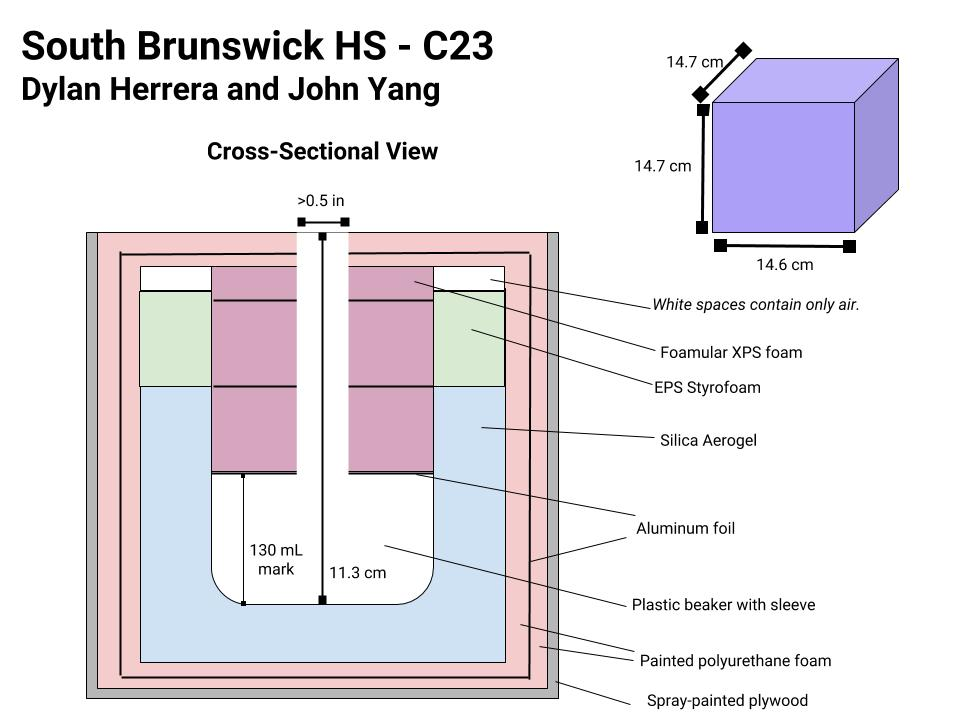
\includegraphics[scale=0.25]{diagram.jpg}
\end{figure}

\subsection{Building and Design}
Research will be required to determine the best material to use in your device. Many teams have found success with products such as aerogel, XPS foam, EPS foam, and polyurethane foam. It will also be good to use a rigid material such as acrylic for the outside of your device, so that everything is neatly contained and you can avoid measurement penalties. Check the resources article for links to different materials. 

\subsection{Calibration}
After building your device, you MUST test it! Other than the 4 required graphs, you should be doing much, much more. Depending on which competitions you go to, you will have to vary a combination of temperature, time, and volume. I recommend setting a time scale of 0, 1, 5, 10, 15, 20, 21, 22, 23, 24, 25, 26, 27, 28, 29, 30. You will have to commit a LARGE amount of time to this event. Calibration of your device will help you make accurate predictions, which is more important than how well your device retains heat. 

\subsection{Equipment}
Although it seems trivial, proper equipment is necessary for your success in this event. I reccomend a glass calibrated thermometer, to ensure that your measurement will be the same as the supervisor's, hoping that they also use a calibrated thermometer. Regarding calculators, choose one that you can use best. The event allows for the use of any calculator, so if you feel that you need a heavy-duty graphing calculator, then use it. However, I only used a simple scientific calculator, and it worked for me. 

\section{The Test}
The 2019 Div. C rules point to the following topics: 1) History, 2) Definition of temperature, Temperature scales and conversions, definitions of heat units, 3) Phases of matter, phase transitions, phase diagrams, latent heat, ideal gas law, 4) Kinds of heat transfer, thermal conductivity, heat capacity, specific heat, 5) Thermodynamic laws and processes (e.g., Carnot cycle and efficiency, adiabatic, isothermal), and 6) Radiant exitance, entropy, enthalpy. While the topics may change when this event comes back, this is a good baseline to start with. \footnotemark Material can be learned conceptually on HyperPhysics. 
\footnotetext{Beware of the Princeton Thermo test}

\subsection{The Binder}
For us, our binder was 1.5" thick. We added sections for all the stuff included in the rules, plus some more. Supervisors will ask questions outside of the scope of the event, so make sure you know about chemical thermodynamics and other topics. Make sure you include a periodic table. For us, there were about 5 or 6 papers we actually used, and everything else was just-in-case we need it. The wikipedia equation table is also a great resource. 
\subsection{History}
History questions tend to be very obscure, and if you don't know, you don't know. Therefore, it is good to read up as much as you can on history. We went on the Wikipedia thermodynamics book, and read about all the scientists listed there. A great binder reference is the wikipedia thermodynamics timeline, which has enough information for you to use on the test, without taking up too much space. Links are provided on the resources document. 

\subsection{Temperature and heat units}
As long as you know these conceptually and quantitatively, you should be fine. Tests tend to ask quesitons about obscure temperature scales, so make sure you look them up and know the conversions. Some tests may also `create' a new temperature scale, so make sure you understand the relation of this to the Zeroth Law of Thermodynamics. 
\subsection{Phases of matter}
Understand the principle behind states of matter, and include a phase diagram of water. know the equation for latent heat $Q=mL$. This type of stuff can be found on Khan academy, which will lead to an adequate understanding of the topic. 
\subsection{Heat Transfer}
For this, you should know about what it says in the rules. Know how to use $Q=mC\Delta T$, and know that $\dfrac{Q}{t}=\dfrac{kA\Delta T}{d}$. Know how to apply these equations, and any others you find on the wikipedia page. Know how to find thermal equilibrium temperature in complex, multi-material systems. 
\subsection{Laws and Processes}
Make sure you know the Carnot Cycle. Know how to draw P-V diagrams and T-S diagrams. You should be able to do this without looking at a reference sheet. In the equation reference sheet, there is a table of equations for different processes. Know how to apply those equations and qualitatively understand the processes and how they are defined. (ex. Isobaric - constant pressure, Isentropic - Constant entropy, etc. )
\subsection{Radiant Exitance, Entropy, Enthalpy}
Know about Blackbody Radiation in general, and know how to use and apply the equation $R=\dfrac{P}{A}=\epsilon\sigma T^4$. For entropy and enthalpy, you should know both the physics side and chem side of it. Know how to find the entropy of an ideal gas, and qualitatively understand it. Be able to identify enthalpy changes in chemical reactions, as well as Gibbs Free Energy and other potentials. \\

Of course, there is always more to be learned, so feel free to use as many resources as you can find. Remember, Google and Wikipedia are your best friends. Good luck!
\end{document}